
%
%  $Description: Author guidelines and sample document in LaTeX 2.09$
%
%  $Author: ienne $
%  $Date: 1995/09/15 15:20:59 $
%  $Revision: 1.4 $
%

\documentclass{sig-alternate}
\usepackage{url}
%\usepackage{times}
%\usepackage{diagrams}
%\usepackage[all]{xy}
\usepackage[ruled,vlined]{algorithm2e}
%\usepackage{float}
\input{macros}
%\documentstyle[times,art10,twocolumn,latex8]{article}

%-------------------------------------------------------------------------
% take the % away on next line to produce the final camera-ready version
\pagestyle{empty}

%-------------------------------------------------------------------------
\begin{document}

%\conferenceinfo{ICSE}{'10, May 2-8 2010, Cape Town, South Africa}
%\CopyrightYear{2010}
%\crdata{978-1-60558-719-6/10/05}


\title{Automated Testing of API Mapping Relations}

%\author{
%Hao Zhong$^{1,2}$\thanks{Corresponding authors}, Suresh Thummalapenta$^4$, Tao Xie$^{4*}$\\
%\small{$^1$Laboratory for Internet Software Technologies, Institute of Software, Chinese Academy of Sciences, Beijing, 100190, China}\\
%\small{$^2$Key Laboratory of High Confidence Software Technologies (Peking University), Ministry of Education, China}\\
%\small{$^3$Institute of Software, School of Electronics Engineering and Computer Science, Peking University, China} \\
%\small{$^4$Department of Computer Science, North Carolina State University, Raleigh, NC 27695-8206, USA}\\
%\small{zhonghao@itechs.iscas.ac.cn, \{sthumma,txie\}@ncsu.edu}}
\numberofauthors{2}
\author{
% You can go ahead and credit any number of authors here,
% e.g. one 'row of three' or two rows (consisting of one row of three
% and a second row of one, two or three).
%
% The command \alignauthor (no curly braces needed) should
% precede each author name, affiliation/snail-mail address and
% e-mail address. Additionally, tag each line of
% affiliation/address with \affaddr, and tag the
% e-mail address with \email.
%
% 1st. author
\alignauthor
Hao Zhong\\
       \affaddr{Laboratory for Internet Software Technologies}\\
       \affaddr{Institute of Software}\\
       \affaddr{Chinese Academy of Sciences, China}\\
       \email{zhonghao@nfs.iscas.ac.cn}
% 2nd. author
\alignauthor
Suresh Thummalapenta and Tao Xie\\
       \affaddr{Department of Computer Science}\\
       \affaddr{North Carolina State University}\\
       \affaddr{Raleigh, NC 27695-8206, USA}\\
       \email{\{sthumma,txie\}@ncsu.edu}
}
\maketitle
\thispagestyle{empty}

\begin{abstract}
Application Programming Interface (API) mapping describes mapping relations of APIs provided by two languages. With API mapping, migration tools are able to translate client code that uses APIs from one language into another language. However, given the same inputs, two mapped APIs can produce different outputs. The different behaviors introduces defects in translated code silently since translated code may have no complication errors. In this paper, we propose an approach, called TeMaAPI (\textbf{Te}sting \textbf{Ma}pping relations of \textbf{API}s), that detects different behaviors of mapped APIs via testing. To detect different behaviors, the test oracle of TeMaAPI is that two mapped APIs should produce the same outputs given the same inputs. Based on our approach, we implement a tool and conduct evaluations on migration tools such as Java2CSharp and Tangible C\# to Java convertor. The results show that TeMaAPI detects ?? different behaviors between mapped APIs of Java2CSharp and ?? different behaviors between mapped APIs of Tangible C\# to Java convertor.
\end{abstract}\vspace*{-2ex}
%% A category with the (minimum) three required fields
%\category{D.2.13 Reusable Software}{Reusable Software}{Reusable libraries}\vspace*{-2ex}
%%A category including the fourth, optional field follows...
%\terms{API mapping relation, Language migration}\vspace*{-2ex}

\section{Introduction}

\label{sec:introduction}

Access control is one of the most fundamental and widely used
security mechanisms. It controls which principals (users, processes,
etc.) have access to which resources in a system. To better manage
access control, systems often explicitly specify access control
policies using policy languages such as XACML~\cite{oasis05:xacml}
and Ponder \cite{damianou01:ponder}. Whenever a principal requests
access to a resource, that request is passed to a software component
called a Policy Decision Point (PDP). PDP evaluates the request
against access control policies, and grants or denies the request
accordingly.

The specification of access control policies is often a challenging
problem. It is common that a system's security is compromised due to
the misconfiguration of access control policies instead of the
failure of cryptographic primitives or protocols. This problem
becomes increasingly severe as software systems become more and more
complex, and are deployed to manage a large amount of sensitive
information and resources that are organized into sophisticated
structures.

Formal verification is an important means to ensuring the correct
specification of access control
policies\Comment{~\cite{jajodia97:logical, sandhu99:arbac}}.
Recently, several tools have been developed to verify XACML access
control policies against user-specified
properties~\cite{hughes04:automated,fisler05:verification,zhang05:evaluating}.
However, it is often beyond the capabilities of these tools to
verify complex access control policies in large-scale information
systems. Furthermore, user-specified properties are often not
available~\cite{fisler05:verification}.

Like in software development, errors in access control policies may
also be discovered through testing. In fact, once access control
policies are specified, they are often tested with some access
requests so that security officers may manually check the PDP's
responses against expected ones~\cite{anderson02:xacml}. However,
current policy testing practice tends to be ad hoc. Although there
exist various coverage criteria~\cite{zhu97:software} for software
programs, there are no criteria or good heuristics to guide
systematic generation of high-quality policy test suites. With an ad
hoc policy testing, it is questionable that high confidence could be
gained on the correctness of access control policies.

This paper presents a first step toward systematic policy testing.
We propose the concept of \Intro{policy coverage} to measure the
quality of policy test suites, which are sets of request-response
pairs. Intuitively, the more policy rules (as well as their
components such as subjects, resources, and conditions) are involved
when evaluating a test suite, the more likely it is to discover
errors in access control policies. We have developed a
coverage-measurement tool to measure the coverage of XACML policies
achieved by a set of access requests. We have also developed a
request-generation tool that randomly generates policy test suites
for a given set of policies.

Although the randomly generated test suites can achieve high policy
coverage, and are effective in detecting a variety of policy
specification errors, it may potentially include a huge number of
requests, which makes it difficult to efficiently inspect and verify
the correctness of responses from the PDP. To mitigate this problem,
we further propose a request reduction technique to significantly
reduce the size of a test suite while maintaining its policy
coverage.

Previous experiments~\cite{rothermel98:empirical} showed that test
reduction based on program code coverage can severely compromise the
fault-detection capabilities of the original test suite. To evaluate
the impact of the proposed request reduction technique on the
quality of policy testing, we conduct an experiment on a set of real
policies with mutation testing~\cite{demillo78:hints}, which is a
specific form of fault injection that consists of creating faulty
versions of a policy by making small syntactic changes. In the
experiment, we compare the fault-detection capabilities of the
reduced set and original set of requests. Our experimental results
show that our coverage-based request reduction technique can
substantially reduce the size of generated requests but incur only
relatively low loss in fault detection capabilities. We also conduct
a study that measures the policy coverage of an XACML conformance
test suite as well as a conference reviewing system's policy. Our
results show that the measurement of policy coverage can effectively
identify uncovered parts of policies. Such results can be used to
guide the development of further test cases, significantly improving
the quality of policy testing.

\Comment{ This paper makes the following main contributions:
\begin{itemize}
\item We propose the concept of policy coverage based on
a general access control model. We further instantiate this
concept in the context of XACML, a widely used and standardized
meta policy language
for expressing domain-specific access control requirements.

\item We develop a coverage-measurement tool for automatically
measuring the coverage for XACML policies achieved by a given set
of requests.

\item We develop a request-generation tool for randomly generating
requests for XACML policies and a request-reduction tool for
greedily selecting a minimal set of requests for achieving the
same policy coverage as the original set of requests.

\item We develop initial mutation operators for XACML policies to
conduct mutation testing. We conduct an experiment on a set of
real policies to compare the effectiveness of the minimal set of
requests with the original set of requests in terms of fault
detection. We also conduct a study on policy coverage of existing
manually generated requests.

\end{itemize}
}

The rest of the paper is organized as follows. Section
\ref{sec:xacml} presents background information on XACML, a widely
used and standardized meta policy language for expressing
domain-specific access control requirements.
Section~\ref{sec:model} proposes the concept of policy testing and
policy coverage based on a general access control model. In
Section~\ref{sec:coverage}, we instantiate the concept of policy
coverage in the context of XACML. We also present the design of a
coverage measurement tool. Sections~\ref{sec:reqgen}
and~\ref{sec:reqreduce} describe the request-generation tool and
our request reduction technique, respectively.
Section~\ref{sec:mutation} presents a set of initial mutation
operators developed for policies. Section~\ref{sec:experiment}
presents the experiment conducted to assess request reduction and
its effect on fault detection capabilities.
Section~\ref{sec:experimentalresults} illustrates the study of
measuring the policy coverage achieved by manually generated
requests. Section~\ref{sec:related} discusses related work and
Section~\ref{sec:conclusion} concludes the paper with future
directions.

















\sloppy

\section{Definitions}
\label{sec:mapping}

We next present definitions of terms used in the rest of the paper.

\textbf{API.} An Application Programming Interface (API)~\cite{orenstein2000quickstudy}
is a set of classes and methods provided by frameworks or libraries.

\textbf{API library.} An API library is a framework
or library that provides reusable API classes and methods.

\textbf{Client code.} Client code is application code
that reuses or extends API classes and methods provided by API
libraries.

The definitions of API library and client code are
relative to each other. For example, Lucene uses
J2SE\footnote{\url{http://java.sun.com/j2se/1.5.0/}} as an API
library, whereas Nutch\footnote{\url{http://lucene.apache.org/nutch/}} uses Lucene as
an API library. Therefore, we consider Lucene as client code and API
library for the J2SE API library and Nutch, respectively. In
general, for programmers of client code, source files of API libraries are often
not available.

\textbf{Mapping relation.} For a set of entities $E_1$ defined by a
language $L_1$ and another set of entities $E_2$ defined by another
language $L_2$, a mapping relation is a triple $\langle E_1, E_2,
b_i \rangle$ where $E_1$ and $E_1$ have the same behavior $b_i$.


We use mapping relations of API classes for translating data such as
variables, parameters, and constants, so we require that two mapped
API classes have the same programm behavior, referred to as
the $s$ behavior.

\textbf{1-to-1 mapping relation of API classes.} For an API class
$c_1$ defined by $L_1$ and an API class $c_2$ defined by $L_2$, a
1-to-1 mapping relation of API classes is a triple $\langle c_1,
c_2, s \rangle$, where $s$ denotes the $s$ behavior.

One API class defined by $L_1$ can have more than one 1-to-1 mapping
relation with API classes defined by $L_2$. For example, data in
\CodeIn{java.util.ArrayList} of Java can be stored in either
\CodeIn{System. Collections.ArrayList} \textbf{or}
\CodeIn{System.Collections.Generic. List} of C\#, so the Java class
has two 1-to-1 mapping relations with the two C\# classes.

\textbf{Many-to-many mapping relation of API classes.} For a set of API classes
$C_1$ defined by $L_1$ and a set of API classes $C_2$ defined by
$L_2$, a many-to-many mapping relation of API classes is a triple
$\langle C_1, C_2, s \rangle$, where $s$ denotes the $s$ behavior.

For example, the current time in \CodeIn{java.lang.System} of Java
is stored in \CodeIn{System.Environment} of C\#, whereas the
environment settings in \CodeIn{java.lang.System} is stored in
\CodeIn{System.Environment} of C\#, so the Java class has a
many-to-many mapping relation with the two C\# classes.

We use mapping relations of API methods for translating API methods
that accept inputs to produce desirable outputs, so we require two
mapped API methods have the same programm behavior of inputs, outputs, and
functionalities. We refer to this behavior as the ``\emph{t}'' behavior.

\textbf{1-to-1 mapping relation of API methods.} For an API method
$m_1$ defined by $L_1$ and an API method $m_2$ defined by
$L_2$, a mapping relation of API methods is a triple $\langle m_1,
m_2, t \rangle$, where $t$ denotes the $t$ behavior.

As one API class defined by $L_1$ can have more than one 1-to-1 mapping
relation with API classes defined by $L_2$, one API method defined by $L_1$ can have more than one 1-to-1 mapping relation with API methods defined by $L_2$. 

\textbf{Many-to-many mapping relation of API classes.} For a set of API methods
$M_1$ defined by $L_1$ and a set of API methods $M_2$ defined by
$L_2$, a many-to-many mapping relation of API methods is a triple
$\langle M_1, M_2, t \rangle$, where $t$ denotes the $t$ behavior.

For example, Section~\ref{sec:introduction} shows a many-to-many mapping relation between $\{m_3\}$ of Java and $\{m_4, m_5\}$ of C\#. 
\section{Example}
\label{sec:example}

\begin{figure*}[t]
\centering
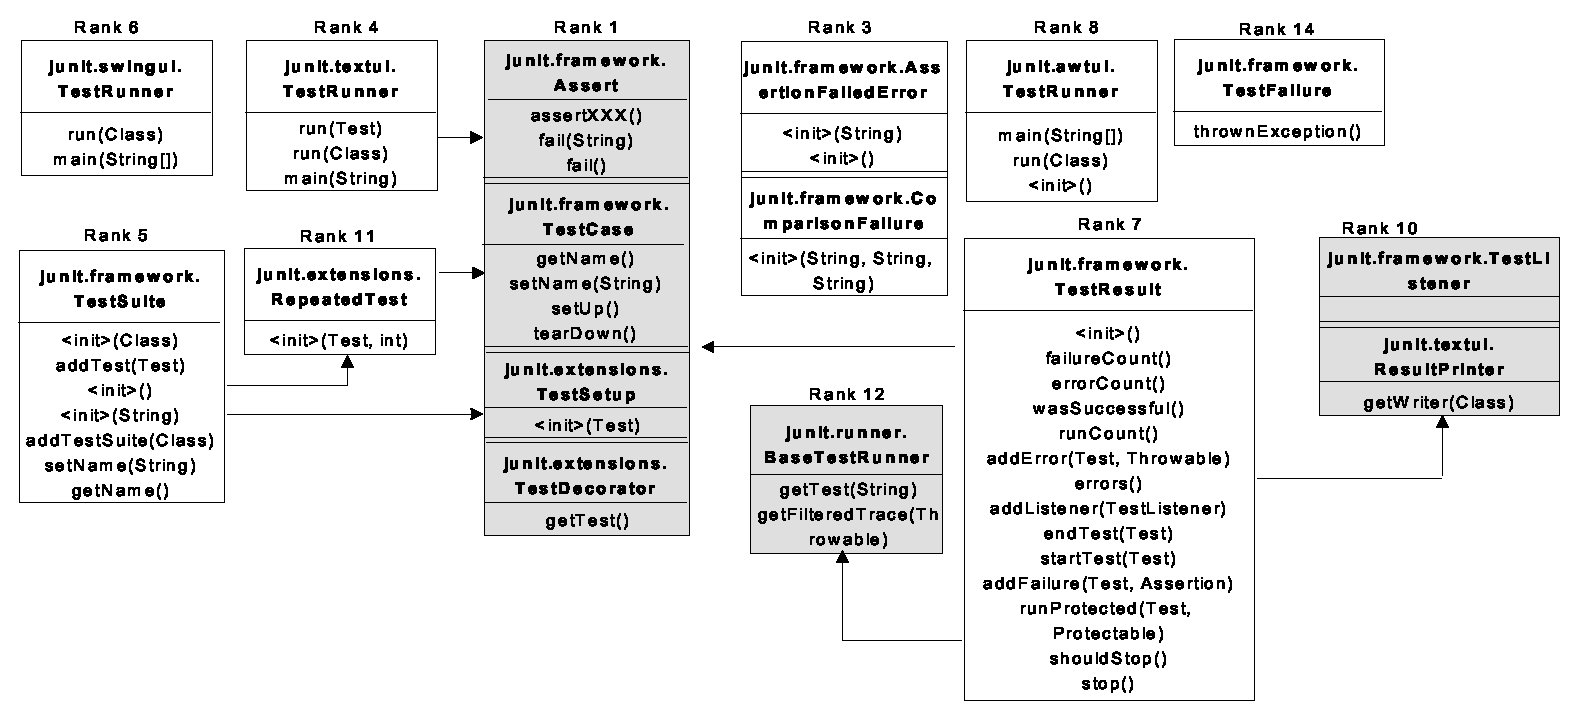
\includegraphics[scale=0.68,clip]{figs/examplehotspot_final.eps}
\caption{Hotspot hierarchies identified for the JUnit framework} \label{fig:hotspotexample}
\end{figure*}

We next use an example to explain our approach and show how the detected
hotspots and coldspots can be used by the framework users. We use JUnit~\cite{JUNIT}, the
\emph{de facto} standard unit testing framework for Java, 
as an illustrative example for explaining our approach.

SpotWeb accepts an input framework, say JUnit, and extracts
\emph{FrameworkInfo} from the framework. The
\emph{FrameworkInfo} includes all classes, all interfaces, public
or protected methods of each class and interface, and inheritance
hierarchy among classes or interfaces of the framework. SpotWeb also captures
the constants defined by the input framework. SpotWeb
constructs different queries for each class or interface and
interacts with a CSE such as Google code search~\cite{GCSE} to
gather relevant code examples from existing open source projects that
reuse the classes of the input framework. For example, SpotWeb constructs
a query such as ``\CodeIn{lang:java junit.framework.TestSuite}'' for
gathering relevant code examples of the \CodeIn{TestSuite} class. These
gathered code examples are referred as a \emph{LocalRepository} for
the input framework. SpotWeb analyzes gathered code examples
statically and computes \emph{UsageMetrics} for classes, interfaces,
and public or protected methods of all classes and interfaces. For
example, the \emph{UsageMetrics} computed for the \CodeIn{TestSuite}
class show that the class is instantiated for 165 times and is
extended for 32 times. Similarly, the \emph{UsageMetrics} computed
for the method \CodeIn{addTest} of the \CodeIn{TestSuite} class show
that the method is invoked for 95 times. SpotWeb also gathers code
examples for each class or method and stores these code examples in
a repository, referred as \emph{ExampleDB}. Then SpotWeb uses the
algorithm shown in Figure~\ref{alg:hotspotalgo} for detecting
hotspots from the computed \emph{UsageMetrics}.

Initially, SpotWeb ranks methods in a non-ascending order based on
their \emph{UsageMetrics} and uses a threshold percentage $HT$ to
detect hotspot methods: the methods in the top $HT$ percentage with
a non-zero \emph{UsageMetrics} are detected as hotspot methods. 
The detected hotspot methods are then
grouped into their declaring classes, detected as hotspot classes.
These hotspot classes are ranked based on the minimum rank of the
hotspot methods declared by these classes. SpotWeb classifies the
hotspot classes into two categories (templates and hooks) based on
heuristics described in Step 4 of the algorithm shown in Figure~\ref{alg:hotspotalgo}. The hotspot classes of each
category are further grouped into hierarchies based on their
inheritance relationships. For example, SpotWeb detected classes
\CodeIn{Assert} and \CodeIn{TestCase} as hook hotspots in the JUnit
framework. As \CodeIn{TestCase} class extends \CodeIn{Assert} class,
SpotWeb groups both the classes into the same hierarchy. SpotWeb
assigns a rank to each hierarchy based on the minimum rank of the
hotspot classes contained in the hierarchy. For example, consider
that the \CodeIn{Assert} class has Rank 1 and the \CodeIn{TestCase}
class has Rank 2, then the grouped hierarchy of the
\CodeIn{Assert} and \CodeIn{TestCase} classes is assigned with Rank
1. The rank attribute uniquely identifies a hierarchy among all
other hierarchies. Hierarchies with smaller ranks have higher preference
or importance to the hierarchies with larger ranks.

Figure~\ref{fig:hotspotexample} shows the hotspot hierarchies detected for the JUnit
framework. The figure also shows ranks assigned to each hierarchy.
As the rank attribute uniquely identifies a hierarchy, we use the
rank as an identity for describing a hierarchy.
Each hierarchy includes one or more hotspot classes and is shown as pairs of class and its methods.
For example, Hierarchy 1 (hierarchy with Rank 1) has classes \CodeIn{Assert}, \CodeIn{TestCase}, \CodeIn{TestSetup},
and \CodeIn{TestDecorator}. We show template hierarchies in white and hook hierarchies in gray.
For example, Hierarchy 1 is a hook hierarchy and Hierarchy 3 is a template hierarchy.

Methods inside each class of a hierarchy are sorted
based on their computed \emph{UsageMetrics}. Sorting methods of a class
can assist the framework users in quickly identifying the methods that are often
used inside a given hotspot class. For example, consider the \CodeIn{TestSuite} class
shown in Hierarchy 5. The \CodeIn{TestSuite} class has three constructors \CodeIn{<init>(Class)},
\CodeIn{<init>()}, and \CodeIn{<init>(String)}. However, the \CodeIn{<init>(Class)} constructor
is often used compared to the other two constructors. Due to space limit,
we show all assertion methods such as \CodeIn{assertEquals} and \CodeIn{assertTrue}
of the class \CodeIn{Assert} of Hierarchy 1 as \CodeIn{assertXXX}.

The figure also displays dependencies among hotspot hierarchies
(shown as arrows between hierarchies). SpotWeb captures the
usage relationships among hotspot classes through dependencies.
For example, Hierarchy $5$ has a
\CodeIn{TEMPLATE\_HOOK} dependency with Hierarchy $1$. This
dependency indicates that to reuse methods such as \CodeIn{addTest}
of the class \CodeIn{TestSuite} in Hierarchy 5, the user has to
define a new behavior for the classes in Hierarchy $1$.

\begin{figure}[t]
\begin{CodeOut}
\begin{alltt}
01:public class SRDAOTestCase 
02:\hspace*{0.4in}extends TestCase \{
03:\hspace*{0.1in}private SRDAO dao = null;...
04:\hspace*{0.1in}public SRDAOTestCase() \{
05:\hspace*{0.3in}super(); ... 
06:\hspace*{0.1in}\}
07:\hspace*{0.1in}protected void setUp() throws Exception \{
08:\hspace*{0.3in}...
09:\hspace*{0.3in}dao = (SRDAO)context.getBean("SRDAO");
10:\hspace*{0.3in}...
11:\hspace*{0.1in}\}
12:\hspace*{0.1in}public void tearDown() throws Exception \{
13:\hspace*{0.3in}dao = null; 
14:\hspace*{0.1in}\}
15:\hspace*{0.1in}public void testF() \{ ... \}
16:\hspace*{0.1in}public void testB() \{ ... \}
17:\hspace*{0.1in}...
18:\}
\end{alltt}
\end{CodeOut}
\Caption{\label{fig:hcodeexample} Suggested code example for the hook class \CodeIn{TestCase}.}
\begin{CodeOut}
\begin{alltt}
01:public class MyTestSuite \{ 
02:\hspace*{0.1in}...
03:\hspace*{0.1in}public static Test suite() \{
04:\hspace*{0.3in}TestSuite suite = new TestSuite("axis");
05:\hspace*{0.3in}suite.addTest(new SRDAOTestCase());
06:\hspace*{0.3in}return suite;
07:\hspace*{0.1in}\}
08:\hspace*{0.1in}...
09:\}
\end{alltt}
\end{CodeOut}
\Caption{\label{fig:tcodeexample} Suggested code example for the template class \CodeIn{TestSuite}.}
\end{figure}

We next describe how the hotspots detected by SpotWeb can be used by
the framework users to reuse classes of the JUnit framework. After reviewing
the hotspots shown in Figure~\ref{fig:hotspotexample}, consider that
a framework user wants to start with the method \CodeIn{addTest} of
the template class \CodeIn{TestSuite} in Hierarchy 5.
Figure~\ref{fig:hotspotexample} shows that Hierarchy 5 of the
\CodeIn{TestSuite} class has a \CodeIn{TEMPLATE\_HOOK} dependency
with the Hierarchy 1. This dependency indicates that the user may
need to define a new behavior for the associated hook hierarchy.
SpotWeb recommends the code example shown in
Figure~\ref{fig:hcodeexample} for the hook class \CodeIn{TestCase},
which is part of Hierarchy 1. The code example exhibits several
aspects that need to be handled by the user while extending the
\CodeIn{TestCase} class. For example, in the \CodeIn{setUp} method,
the user can write code for setting up the environment such as
instantiating necessary variables, and in the \CodeIn{tearDown}
method, the user can destroy the created variables. In addition, the code
example shows that names of the test methods in the extended class
of the \CodeIn{TestCase} class should start with the prefix \CodeIn{test}.
SpotWeb also recommends a code example for the \CodeIn{addTest} method and
the recommended code example is shown in
Figure~\ref{fig:tcodeexample}. The code example shows that the user
has to create an instance of the \CodeIn{TestSuite} class and then
add test cases through the \CodeIn{addTest} method.

An API class or method is identified as a coldspot if that class or method is neither
used directly nor used indirectly by gathered code examples. The complete
algorithm used for detecting coldspots is shown in Figure~\ref{alg:coldspotalg}. SpotWeb identified $20$
classes such as \CodeIn{Swapper}, \CodeIn{TestRunListener}, and \CodeIn{ExceptionTestCase} as coldspots
in the JUnit framework. However, coldspots are only suggestions
for users unfamiliar to that framework and SpotWeb does not intend to recommend users not to reuse
those coldspot classes. Sometimes, coldspots can also be helpful to
the framework developers in distributing their maintenance efforts, because the framework
developers can give a low preference to the coldspot classes.
\vspace*{-1ex}
\section{Approach}
\label{sec:approach}
\begin{figure}[t]
\centering
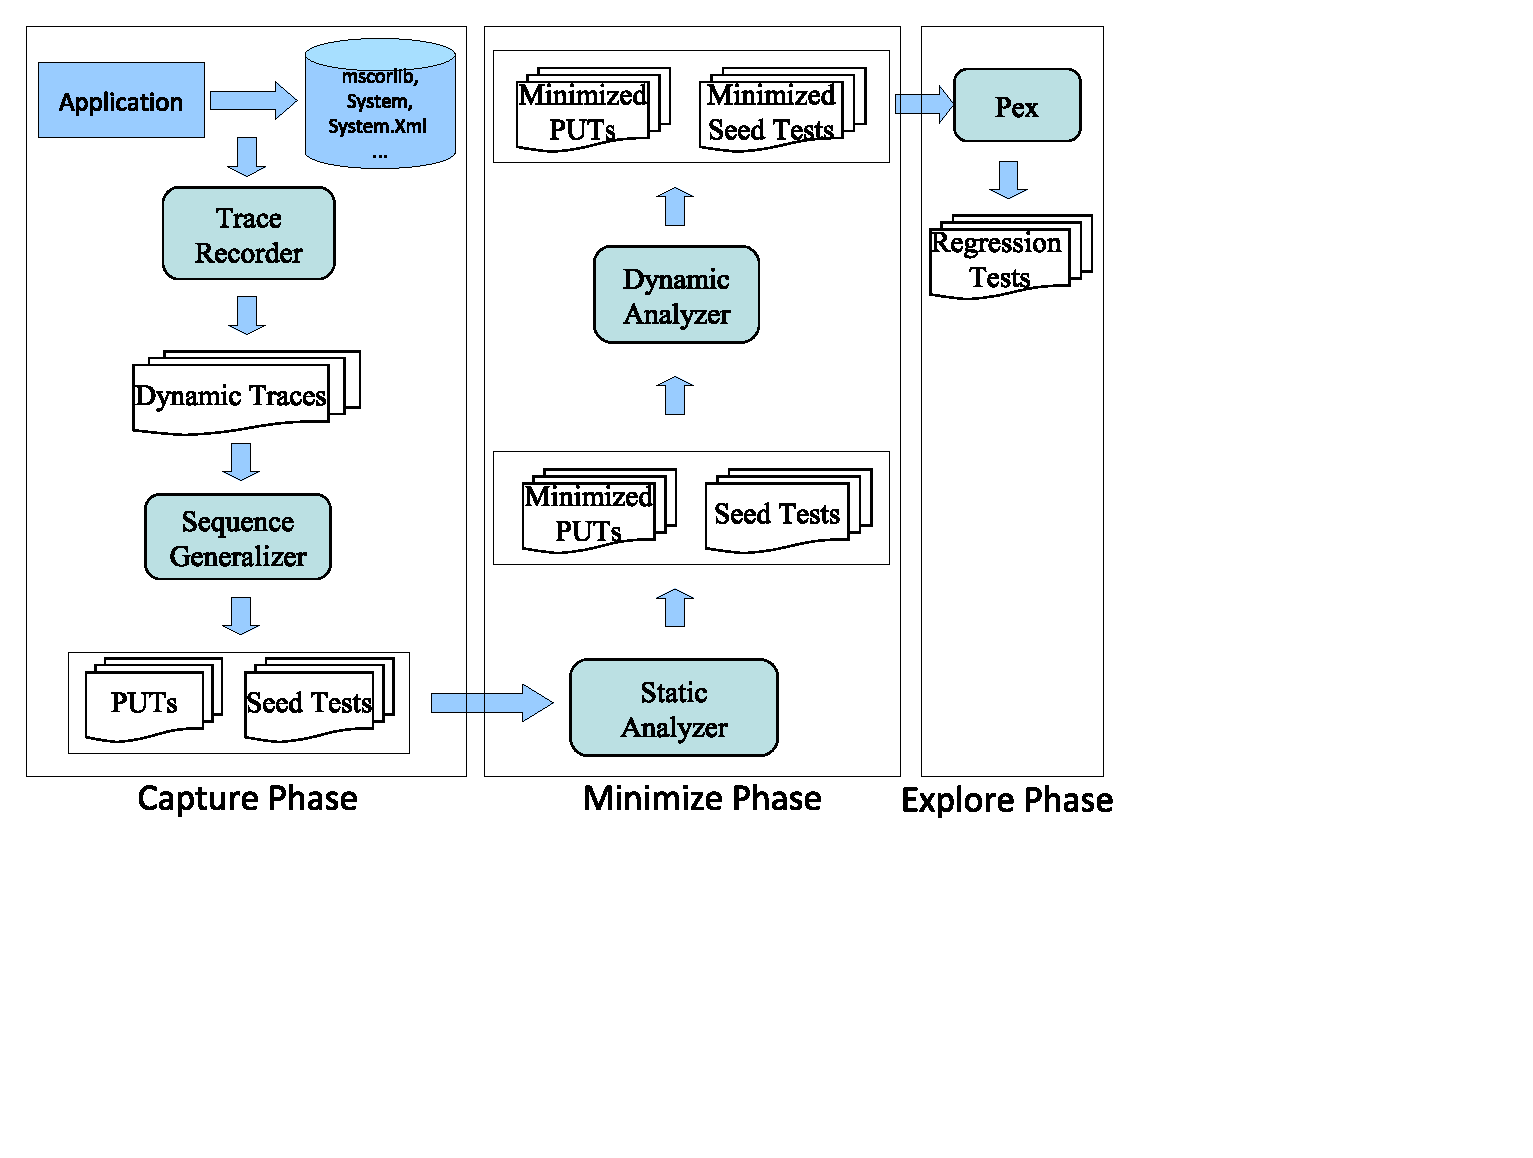
\includegraphics[scale=1,clip]{figure/approach.eps}\vspace*{-3ex}
 \caption{Overview of TeMaAPI}\vspace*{-4ex}
 \label{fig:approach}
\end{figure}
Given a migration tool between Java and C\#, TeMaAPI generates various test cases to reveal different behaviors of the tool's API mapping relations.
Figure~\ref{fig:approach} shows the overview of TeMaAPI.


%-------------------------------------------------------------------
\subsection{Generating client code}
\label{sec:approach:generating}
Given a migration tool, TeMaAPI first extracts its validate mapping relations of APIs. It is challenging to extract such mapping relations directly from a migration tool for two factors: (1) different migration tools may follow different styles to describe API mapping relations. For example, as shown in Section~\ref{sec:introduction}, the API mapping relations of Java2CSharp are described in its mapping files, but the API mapping relations of sharpen are hard-coded in its source files. (2) commercial migration tools typically hide their API mapping relations in binary files. Due to the two factors, TeMaAPI does not extract API mapping relations directly from a migration tool, but chooses to analyze translated code of a migration tool. We choose to use migration tools to translate simple client code instead of existing projects for two considerations: (1) Existing projects typically use quite a small set of APIs, so many API mapping relations may be not covered; (2) a single method of an existing project may use multiple APIs, so it may be difficult to analyze which APIs are not mapped. For the preceding consideration, TeMaAPI chooses to generate client code instead of using existing client code.

TeMaAPI relies on the reflection technique~\cite{maes1987concepts} provided by both Java and C\# to generate client code for translation.

\textbf{Static fields.} Given a public static field \CodeIn{f} of a class \CodeIn{C} whose type is \CodeIn{T}, TeMaAPI generates a getter as follows:
\begin{CodeOut}%\vspace*{-2ex}
\begin{alltt}
 public T TestGet|f.name||no|()\{ return C.f; \}
\end{alltt}
\end{CodeOut}

If \CodeIn{f} is not a constant, TeMaAPI generates a setter as follows:
\begin{CodeOut}%\vspace*{-2ex}
\begin{alltt}
 public void TestSet|f.name||no|(T v)\{ C.f = v; \}
\end{alltt}
\end{CodeOut}

\textbf{Non-static fields.} Given a public non-static field \CodeIn{f} of a class \CodeIn{C} whose type is \CodeIn{T}, TeMaAPI generates a getter for each constructor \CodeIn{C(T1\ p1,\ldots, Tn\ pn)} of \CodeIn{C} as follows:
\begin{CodeOut}%\vspace*{-2ex}
\begin{alltt}
 public T TestGet|f.name||no|(T1\ c1,\ldots, Tn\ cn)\{
    C obj = new C(c1,\ldots, cn);
    return obj.f; \}
\end{alltt}
\end{CodeOut}

If \CodeIn{f} is not a constant, TeMaAPI generates a setter as follows:
\begin{CodeOut}%\vspace*{-2ex}
\begin{alltt}
 public void TestSet|f.name||no|(T1\ c1,\ldots, Tn\ cn)\{
   C obj = new C(c1,\ldots, cn);
   obj.f = v; \}
\end{alltt}
\end{CodeOut}

In the preceding code, ``\CodeIn{|f.name|}'' denotes the name of \CodeIn{f}, and ``\CodeIn{|no|}'' denotes the corresponding number of generated client-code method.

\textbf{Static methods.} Given a public static method \CodeIn{m(T1\ p1,\ldots,Tn\ pn)} of a class \CodeIn{C} whose return type is \CodeIn{Tm}, TeMaAPI generates a client-code method as follows:
\begin{CodeOut}%\vspace*{-2ex}
\begin{alltt}
 public Tm Test|m.name||no|(T1\ m1,\ldots, Tn\ mn)\{
   return C.m(m1,\ldots, mn); \}
\end{alltt}
\end{CodeOut}

\textbf{Non-static methods.} Given a public non-static method \CodeIn{m(T1\ p1,\ldots,Tn\ pn)} of a class \CodeIn{C} whose return type is \CodeIn{Tm}, TeMaAPI generates a client-code method for each constructor \CodeIn{C(Tv\ pv,\ldots, Tt\ pt)} of \CodeIn{C} as follows:
\begin{CodeOut}%\vspace*{-2ex}
\begin{alltt}
 public Tm Test|m.name||no|(T1\ m1,\ldots, Tn\ mn,
                            Tv cv, \ldots, Tt ct)\{
   C obj = new C(cv,\ldots, ct);
   return obj.m(m1,\ldots, mn); \}
\end{alltt}
\end{CodeOut}

In the preceding code, ``\CodeIn{|m.name|}'' denotes the name of \CodeIn{m(T1\ p1,\ldots,Tn\ pn)}.

TeMaAPI ignores generic methods for simplicity, and organizes all generated client code methods by the corresponding class $C$. For a migration tool that translates from Java to C\#, TeMaAPI generates client code in Java as shown by the solid line of Figure~\ref{fig:approach}, and for a migration tool that translates from C\# to Java, TeMaAPI generates client code in C\# as shown by the dotted line of Figure~\ref{fig:approach}. When TeMaAPI generates client code in C\#, it ignores \CodeIn{unsafe} and \CodeIn{delegate} methods and methods whose parameters are marked as \CodeIn{our} or \CodeIn{ref}. Java does not have corresponding keywords, so there are typically no mapped methods in Java for these C\# methods. After TeMaAPI generate client-code methods, we translate them using a migration tool under experiments.


%-----------------------------------------------------------------
\subsection{Analyzing Generated Methods}
\label{sec:approach:analyzing}
Translated code typically contain many compilation errors since a migration tool typically cannot cover mapping relations of all APIs. TeMaAPI then analyzes translated code for validate API mapping relations of the migration tool. To achieve this, TeMaAPI first remove all translated methods with compilation errors. For translated methods in Java, TeMaAPI implements a Eclipse plug-in that uses on Eclipse JDT compiler\footnote{\url{http://www.eclipse.org/jdt/}} for the list of compilation errors. For translated methods in C\#, TeMaAPI implements a Visual Studio.Net add-in to retrieve the list of compilation errors from the error-list view of Visual Studio.Net. Both Eclipse JDT compiler and Visual Studio.Net cannot list all methods with compilation errors in a single build. After each iteration of removing methods, TeMaAPI re-build these methods until it removes all methods with compilation errors.

After methods with compilation errors are removed, TeMaAPI compares generated code with translated code for the validate API mapping relations of a migration tool. Based on translated code and validate API mapping, TeMaAPI removes generated methods whose corresponding translated methods have compilation errors. We refer to those removing client-code methods as safe methods.

%-----------------------------------------------------------
\subsection{Finding Different Behaviors}
\label{sec:approach:behavior}
In the final step, TeMaAPI generates test cases to detect different behaviors of API mapping relations. An alternative approach is to use existing test cases in two languages. For example, lucene\footnote{\url{http://lucene.apache.org}} has both a Java version and a C\# version. It is feasible to use these test cases to reveal some different behaviors, but such test cases typically cover only a small set of APIs. Some test suites such as Java Compatibility Kit (JCK)\footnote{\url{http://jck.dev.java.net}} cover most APIs of a language. However, translating such a test suite from one language into another language may introduce many compilation errors and defects. A test method may use many APIs, so even if the API under test can be translated correctly, the test method cannot be translated correctly since other APIs are not mapped. As a result, we choose to translating existing test suites as a supplement of our approach.

\subsubsection{Generating Test Cases}
\label{sec:approach:behavior:generating}
For each safe method in Java, we use Randoop~\cite{pacheco2007feedback} to generate its test cases. For each safe method in C\#, we use Pex~\cite{tillmann2008pex} to generate its test cases. TeMaAPI then executes generated test cases, and records the inputs, the output, and the thrown exception of each test case as a file.

Based on the file, TeMaAPI generates Junit\footnote{\url{http://www.junit.org/}} or Nunit\footnote{\url{http://www.nunit.org/}} test cases to ensure each mapped API produce the same output give the same inputs. For example, Pex generates a test case whose input is \CodeIn{m0 = false} for the \CodeIn{TestvalueOf57} method in C\# as shown in Section~\ref{sec:example}, and after executing the output of the test case is ``False''. Based on the input and the output of this test case, TeMaAPI generates a Junit test case as follows:

\begin{CodeOut}%\vspace*{-2ex}
\begin{alltt}
 @Test
 public void testvalueOf64zhh0()\{
   sketch.Test_java_lang_String obj =
                       new sketch.Test_java_lang_String();
   boolean m0 = false;
   Assert.assertEquals("False", obj.testvalueOf64(m0));\}
\end{alltt}
\end{CodeOut}

This Junit test case fails since the preceding \CodeIn{testvalueOf64zhh} method produces ``false'' instead of ``False''. From this failed Junit test case, TeMaAPI detects that the \CodeIn{java.lang.String.valueOf (Object)} method in Java has different behaviors with its mapped C\# methods if inputs are boolean values.

In some cases, executing a test case does not produce outputs but exceptions. For example, Pex also generates a test case whose input is \CodeIn{m0 = null} for the \CodeIn{TestvalueOf57} method in C\# as shown in Section~\ref{sec:example}, after executing it throws \CodeIn{NullReferenceException}. TeMaAPI finds that the \CodeIn{NullPointerException} class in C\# is mapped to the \CodeIn{NullPointerException} class in Java in the validate API mapping relations, and generates a Junit test case based on the preceding mapping relation and input as follows:

\begin{CodeOut}%\vspace*{-2ex}
\begin{alltt}
 @Test
 public void testvalueOf64zhh3()\{
   try\{
     sketch.Test_java_lang_String obj =
                       new sketch.Test_java_lang_String();
     boolean m0 = null;
     obj.testvalueOf64(m0);\}
   \}catch(java.lang.NullPointerException e)\{
       Assert.assertTrue(true);
       return;
   \}
   Assert.assertTrue(false);\}
\end{alltt}
\end{CodeOut}

This Junit test case also fails since given a null input, the preceding \CodeIn{testvalueOf64} method does not throw any exceptions. From this failed Junit test case, TeMaAPI detects that the \CodeIn{java.lang. String.valueOf(Object)} method in Java has different behaviors with its mapped C\# methods if inputs are null pointers.

\subsubsection{Translating Existing Test Cases}
\label{sec:approach:behavior:jck}

Each generated client-code method uses only one fields or methods provided by API libraries, and may lose some complicated behaviors even if test cases satisfy the round-trip criterion. To test those complicated behaviors, we introduce JCK that covers many complicated behaviors of Java APIs. JCK is a test suite provided by Sun to ensure compatibility of Java platforms, and it covers most standard APIs of J2SE. However, JCK implements many internal classes to collect the results of executed test cases. If a migration tool cannot correctly translate one of these classes, all translated test cases may have compilation errors or defects. In addition, JCK is released under read-only source license\footnote{\url{http://tinyurl.com/33x9fo6}}, so many such internal classes are not shipped and it has many compilation errors. To increase the chance of migrating JCK, TeMaAPI first replaces those internal classes with the classes of Junit. For example, one test method for \CodeIn{java.io.File.delete()} in JCK is as follows:

\begin{CodeOut}%\vspace*{-2ex}
\begin{alltt}
  public Status File0037()\{
    String testCaseID = "File0037";
    ...
    FileRT method = new FileRT(testCaseID) \{
     public Status run() \{
       File f = null;
       f = new File(workdir, testCaseID);
       ...
       if (f.delete()) \{ // Try to delete
         if (!f.exists()) \{ // Does it exist?
           return Status.passed("OKAY");
         \}else\{
            return Status.failed(...);
         \}
       else\{
           return Status.failed(...);
       \}
    \}
     return AllPermissionSM.testRun(...);
  \}
\end{alltt}
\end{CodeOut}

After the preceding three steps, TeMaAPI further replaces the statement starts with \CodeIn{FileRT} with the body of the \CodeIn{run} method, and removes the last statement. The translated code is as follows:

\begin{CodeOut}%\vspace*{-2ex}
\begin{alltt}
  public void File0037()\{
    String testCaseID = "File0037";
    ...
    File f = null;
    f = new File(workdir, testCaseID);
    ...
    if (f.delete()) \{ // Try to delete
      if (!f.exists()) \{ // Does it exist?
        Assert.assertTrue(true);
        return;
     \}else\{
        Assert.fail();
        return;
     \}
   else\{
       Assert.fail();
       return;
   \}
  \}
\end{alltt}
\end{CodeOut}

Compared with the original test method in JCK, the translated method does not use the three internal classes: \CodeIn{Status}, \CodeIn{FileRT}, and \CodeIn{AllPermissionSM}. 

After the preceding process, for a migration tool, TeMaAPI further removes methods that use any APIs outside its defined mapping relations. The remaining methods can be translated from Java to other languages since it does not use any APIs outside of the migration tool.


\vspace*{-1ex}
\section{Evaluations}
\label{sec:evaluation}

We implemented a tool for TeMAPI and
conducted evaluations using our tool to address the following
research questions:

%\vspace*{-1.5ex}
\begin{enumerate}
\item How effectively can existing translation tool translate API invocations (Section~\ref{sec:evaluation:invocation})? \vspace*{-1.8ex}
\item How effectively can our approach detect behavior differences of single API invocations (Section~\ref{sec:evaluation:single})?\vspace*{-1.8ex}
\item How effectively can our approach detect behavior differences of multiple API invocations (Section~\ref{sec:evaluation:sequence})?\vspace*{-1.8ex}
\item Can the our combination strategy helps achieve better coverage (Section~\ref{sec:evaluation:coverage})?
\end{enumerate}%\vspace*{-1.5ex}

\begin{table}[t]
\centering
\begin{SmallOut}
\begin {tabular} {|c|l|c|c|c|c|c|c|}
 \hline
\textbf{Name}& \textbf{Version}& \textbf{Provider} &\textbf{Description}\\
\hline
Java2CSharp  &  1.3.4 & IBM (ILOG) & Java to C\# \\
\hline
JLCA         &  3.0   & Microsoft  & Java to C\# \\
\hline
sharpen      &  1.4.6 & db4o       & Java to C\# \\
\hline
Net2Java     &  1.0   & NetBean    &  C\# to Java\\
\hline
VB \& C\# to Java converter    &  1.6   & Tangible   &  C\# to Java\\
\hline
\end{tabular}\vspace*{-2ex}
\Caption{Subject tools} \label{table:subjects}
\end{SmallOut}\vspace*{-2ex}
\end{table}

Table~\ref{table:subjects} shows the subject tools in our evaluation. Column ``Name'' lists the names of subject tools. In the rest of the paper, we call ``VB \& C\# to Java converter'' as converter for short. Column ``Provider'' lists their companies. Although all these tools are developed by commercial companies, Java2CSharp, sharpen, and Net2Java are all open source. Column ``Description'' lists the main functionalities of subject tools. We choose these tools as subjects since we find that many programmer recommend these tools in various forums.

All evaluations were conducted on a PC with Intel Qual CPU @
2.83GHz and 1.98M memory running Windows XP.

\subsection{Translating Generated Wrapper Methods}
\label{sec:evaluation:invocation}
For Java to C\# tools, we use TeMAPI to generate wrapper methods for J2SE 6.0\footnote{\url{http://java.sun.com/javase/6/docs/api/}}. As described in Section~\ref{sec:approach:generating}, TeMAPI ignores all generic API methods. Table~\ref{table:java2csharp} shows the translation results. Column ``Type'' lists the types of generated methods. In particular, ``sfg'' denotes getters of static fields; ``sfs'' denotes setters of static fields; ``nfg'' denotes getters of non-static fields; ``nfs'' denotes setters of non-static fields; ``sm'' denotes static methods; ``nm'' denotes non-static methods; and ``Total'' denotes the sums of all methods. Column ``Number'' lists numbers of corresponding types of methods. Columns ``Java2CSharp'', ``JLCA'', and ``sharpen'' list the translation results of corresponding translation tools. For these columns, sub-column ``M'' lists the number of translated methods without compilation errors, and sub-column ``\%'' lists the percentage from translated method without compilation errors to corresponding generated methods.
\begin{table}[t]
\centering
\begin{SmallOut}
\begin {tabular} {|c|r|r|r|r|r|c|c|}
 \hline
\multirow{2}*[-2pt]{\textbf{Type}}&
\multicolumn{1}{|c}{\multirow{2}*[-2pt]{\textbf{No}}}
& \multicolumn{2}{|c|}{\textbf{Java2CSharp}} & \multicolumn{2}{|c|}{\textbf{JLCA}}& \multicolumn{2}{|c|}{\textbf{sharpen}} \\\cline{3-8} &  &  \textbf{M}& \textbf{\%} &  \textbf{M}& \textbf{\%}&  \textbf{M}& {\%}\\
\hline
sfg  &  16962 & 237 & 1.4\% & 3744 & 22.1\% & 47 & 0.3\%\\
\hline
sfs  &  0    & 0    & n/a   & 0    & n/a    & 0  & n/a  \\
\hline
nfg  &  832  & 0    & 0.0\% & 121  & 14.5\% & 26 & 2.2\%\\
\hline
nfs  &  823  & 0    & 0.0\% & 79   & 9.6\%  & 0   & 0.0\%\\
\hline
sm   &1175   & 97   & 8.3\% & 198  & 16.9\% & 26  & 2.2\%\\
\hline
nm   &175400 & 3589 & 2.0\% & 39536& 22.5\% & 1112& 0.6\%  \\
\hline
Total &195192& 3923 &  2.0\% & 43678 & 22.4\% & 1185 & 0.6\%\\
\hline
\end{tabular}\vspace*{-2ex}
\Caption{Translation results of Java to C\# tools} \label{table:java2csharp}
\end{SmallOut}\vspace*{-2ex}
\end{table}

From the results of Table~\ref{table:java2csharp}, we find that it is quite challenging for a translation tool to cover all API invocations. One challenge lies in that API invocations are quite large in size. Although JLCA can translate 43678 generated methods, it covers only 22.4\% of total generated methods. The other challenge lies in that many API invocations of different languages cannot be accurately mapped. For example, as pointed out by our previous work~\cite{zhong2010mining}, one API method in one language may be mapped to several API methods in another language. We find that all the three translation tools have techniques to deal with many-to-many mapping relations. In particular, Java2CSharp and sharpen develop their own assemblies and map some API invocations to their implemented assemblies instead of standard C\# API invocations. For example, Java2CSharp maps the \CodeIn{java.lang.Class.forName(String)} method in Java to the \CodeIn{ILOG.J2CsMapping.Reflect.Helper.GetNativeType(String)} method in C\#, and the latter method is provided by Java2CSharp. JLCA does not implement additional assemblies, but generate additional source code to hide behavior differences. Although all the three translation tools take the behavior differences of mapped API invocations seriously, they do not cover all differences of API mapping relations. For example, when JLCA translates generated code, it generates a report with 1265 warning messages for behavior differences of API mapping relations. One warning message is ``Method 'java.lang.String.indexOf' was converted to 'System.String.IndexOf' which may throw an exception''. Still, JLCA leaves these differences to programmers, and the report does not tell programmers when such an exceptions is thrown.


\begin{table}[t]
\centering
\begin{SmallOut}
\begin {tabular} {|c|r|r|r|r|r|c|c|}
 \hline
\multirow{2}*[-2pt]{\textbf{Type}}&
\multicolumn{1}{|c}{\multirow{2}*[-2pt]{\textbf{No}}}
& \multicolumn{2}{|c|}{\textbf{Net2Java}} & \multicolumn{2}{|c|}{\textbf{converter}}\\\cline{3-6} &  &  \textbf{M}& \textbf{\%} &  \textbf{M}& \textbf{\%}\\
\hline
sfg  &  3223 & 1    & 0.0\% & 3    & 0.1\% \\
\hline
sfs  &  8    & 0    & 0.0\% & 0    & 0.0\%   \\
\hline
nfg  &  117  & 0    & 0.0\% & 0    & 0.0\%\\
\hline
nfs  &  115  & 0    & 0.0\% & 0    & 0.0\%\\
\hline
sm   &996    & 22   & 2.2\% & 387  & 38.9\% \\
\hline
nm   &190376 & 4    & 0.0\% & 6    & 0.0\% \\
\hline
Total &194835& 27   &  0.0\% & 396 & 0.2\%\\
\hline
\end{tabular}\vspace*{-2ex}
\Caption{Translation results of C\# to Java tools} \label{table:csharp2java}
\end{SmallOut}\vspace*{-2ex}
\end{table}

For C\# to Java translation tools, we use TeMAPI to generate wrapper methods for the .Net framework client profile\footnote{\url{http://tinyurl.com/252t2ax}}. As described in Section~\ref{sec:approach:generating}, besides generic methods, TeMAPI also ignores methods whose parameters are marked with \CodeIn{out} or \CodeIn{ref}. Table~\ref{table:csharp2java} shows the translation results. Columns of Table~\ref{table:csharp2java} are of the same meanings with the columns of Table~\ref{table:java2csharp}. TeMAPI generates almost the same size of methods as it generates for J2SE 6.0. From the results of Table~\ref{table:java2csharp}, we find that both the two tool translate only quite a small portion of API invocations. As described in the wikipedia\footnote{\url{http://tinyurl.com/yj4v2m2}}, C\# provides many features that Java does not have (\emph{e.g.}, partial class, reference parameters, output parameters, and named arguments). We suspect that a C\# to Java translation tool needs take more effects on these issues, so many mapping relations of API invocations are not addressed yet.


Comparing the translation results between Java-to-C\# tools and C\#-to-Java tools, we find that Java-to-C\# tools cover much more API invocations. To fully explore the translation results of Java-to-C\# tools, we present the results of the package level in Table~\ref{table:package}. Column ``Name'' lists the names of Java packages. To save space, we omit the prefixes such as ``java.'', ``javax.'', and ``org.'' if it does not introduce ambiguity. We also use short names for some packages. In particular, we use ``acc.'' to denote the \CodeIn{javax.accessibility} package, ``man.'' to denote the \CodeIn{javax.management} package, ``java. sec.'' to denote the \CodeIn{java.security} package, and ``javax.sec.'' to denote the \CodeIn{javax.security} package. We also omits 12 packages that are not covered by all the three tools (\emph{e.g.}, the \CodeIn{javax.rmi} package). Other columns of Table~\ref{table:package} are of the same meanings with the columns of Table~\ref{table:java2csharp}. From the results of Table~\ref{table:package}, we find that all the three translation tools cover the \CodeIn{java.io} package, the \CodeIn{java.lang} package, the \CodeIn{java.util} package, and the \CodeIn{java.net} package. The four packages may be quite important for most Java programs. Almost for all packages, JLCA covers more API invocations. In particular, JLCA covers GUI-related packages such as the \CodeIn{java.awt} package and the \CodeIn{javax.swing} package. As a result, JLCA can translate some Java programs with GUI interfaces whereas the other two tools cannot.

\subsection{Testing Single Invocations}
\label{sec:evaluation:single}


To test behavior differences of single invocations, TeMAPI leverages Pex to search internal paths for C\# wrapper methods. These methods include the translated C\# methods without compilation errors as shown in Table~\ref{table:java2csharp} and the generated C\# methods that can be translated into Java without compilation errors as shown in Table~\ref{table:csharp2java}. When Pex searches those paths, TeMAPI records the inputs and output of each iteration. Based on these inputs and outputs, TeMAPI generates Java test cases to ensure that the generated methods and the translated methods produce the same outputs given the same inputs. As it requires human interactions to test GUI related API invocations, we filter out GUI related API invocations under the \CodeIn{awt} package and the \CodeIn{swing} package although JLCA is able to translate some GUI related API invocations. In addition, when Pex searches methods without return values, we ignore those paths that do not throw any exceptions since we cannot generate Java test cases for them. We discuss this issue in Section~\ref{sec:discuss}.


We run the generated Java test cases, and Table~\ref{table:singleinvoc} shows the results. Column ``Name'' lists the name of translation tools. Column ``Java'' lists numbers of generated Java test cases. Columns ``Error'' and ``Failure'' list number of test cases that end with errors and failures, respectively. Sub-column ``M'' lists numbers of test cases. Sub-column ``\%'' lists percentages from the numbers of corresponding test cases to the numbers of total generated test cases. From the results of Table~\ref{table:singleinvoc}, we find that totally only about half the generated Java test cases get passed. It turns out that TeMAPI is quite effective to detect behavior differences of mapped API invocations since it searches every paths of methods under test. The results also reflect that the API mapping relations defined in JLCA and sharpen are more reliable than other tools since more test cases of the two tools get passed than other four tools.
\begin{table}[t]
\centering
\begin{SmallOut}
\begin {tabular} {|p{3.6em}|r|r|r|r|r|c|c|}
 \hline
\multicolumn{1}{|c}{\multirow{2}*[-2pt]{\textbf{Name}}}&
\multicolumn{1}{|c|}{\multirow{2}*[-2pt]{\textbf{No}}}
& \multicolumn{2}{|c|}{\textbf{Java2CSharp}} & \multicolumn{2}{|c|}{\textbf{JLCA}}& \multicolumn{2}{|c|}{\textbf{sharpen}} \\\cline{3-8} &  &  \textbf{M}& \textbf{\%} &  \textbf{M}& \textbf{\%}&  \textbf{M}& {\%}\\
\hline
awt  &  29199  & 0     &  0.0\%  &  8637  &  29.6\%  &  0   & 0.0\%\\
\hline
bean &  \hfill 1768   & 20    &  1.1\%  &  14    &  0.8\%   &  0   & 0.0\% \\
\hline
io   &  \hfill 3109   & 592   &  19.0\% & 1642   &  52.8\%  & 43   & 1.4\%\\
\hline
lang &  \hfill 5221   & 1494  &  28.6\% & 2377   &  45.5\%  & 791  & 15.2\%\\
\hline
math &  \hfill 1584   & 101   &  6.4\%  & 232    &  14.6\%  & 0    & 0.0\%\\
\hline
java.net  &  \hfill 1990   & 52    &  2.6\%  & 482    &  24.2\%  & 10   & 0.5\%  \\
\hline
nio  &  \hfill 536    & 30    &  5.6\%  & 0      &  0.0\%  &  0    & 0.0\%  \\
\hline
java.rmi  &  \hfill 1252   & 0     &  0.0\%  &  707   &  56.5\%  &  0   & 0.0\%\\
\hline
java.sec. &  \hfill 2797   & 50    &  1.8\%  &  702    &  25.1\%   &  0   & 0.0\% \\
\hline
java.sql   &  \hfill 3495   & 20   &  0.6\% & 183   &  5.2\%  & 0   & 0.0\%\\
\hline
text  &  \hfill 1068   & 96   &  9.0\% & 321   &  30.1\%  & 0  & 0.0\%\\
\hline
util  &  \hfill 9586   & 1372   &  14.3\%  & 1879    &  19.6\%  & 341    & 3.6\%\\
\hline
acc.  &  \hfill 237   & 1    &  0.4\%  & 25    &  10.5\%  & 0   & 0.0\%  \\
\hline
activation     &  \hfill 538   & 0    &  0.0\%  & 165   &  30.7\%  & 0   & 0.0\%  \\
\hline
crypto        &  \hfill 625   &  0    &  0.0\%  &  263  &  42.1\%  &  0    & 0.0\%\\
\hline
man.   &  \hfill 5380   & 2    &   0.0\%  & 0     &  0.0\%  & 0    & 0.0\%  \\
\hline
naming       &  \hfill 3565   & 0    &   0.0\%  & 1365   &  38.3\%  &  0    & 0.0\%  \\
\hline
javax.sec.       &  \hfill 1435  & 0     &  0.0\%  & 619     &  43.1\%  & 0    & 0.0\%\\
\hline
sound          &  \hfill 515   & 0    &  0.0\%  & 56    &  10.9\%  & 0   & 0.0\%  \\
\hline
swing          &  102389& 10   &  0.0\%  &  21364 &  20.9\%   &  0   & 0.0\%\\
\hline
javax.xml            &  \hfill 4188  &  34   &  0.8\% &  580   &  13.8\%  & 0  & 0.0\%\\
\hline
org.omg              &  \hfill 8937   & 0    &  0.0\%  & 1578  &  17.7\%  & 0   & 0.0\%  \\
\hline
w3c.dom          &  \hfill 83     & 0    &  0.0\%  & 14     &  16.9\%   & 0   & 0.0\%  \\
\hline
org.xml             &   \hfill 897    & 49   &  5.5\%  & 473    & 52.7\%    & 0   & 0.0\%\\
\hline
\end{tabular}\vspace*{-2ex}
\Caption{Translation results of package level} \label{table:package}
\end{SmallOut}\vspace*{-2ex}
\end{table}


For tools such as Java2CSharp, JLCA, and sharpen, we further present their testing results of the package level in Table~\ref{table:packagetest}. Column ``Name'' lists names of J2SE packages. For columns ``Java2CSharp'', ``JLCA'', and ``sharpen'', sub-column ``R'' lists numbers of generated Java test cases, and sub-column ``\%'' lists percentages from the test cases end with errors or failures to the total test cases. From the results of Table~\ref{table:packagetest}, we find that for the \CodeIn{java.sql} package and the \CodeIn{java.util} package, all the tools suffer relatively high error/failure percentages, and for the \CodeIn{java.lang} package and the \CodeIn{java.math} package, all the tools achieve relatively low error/failure percentages. The results may reflect that some packages between Java and C\# are more similar than others, so that they can more easily mapped. We also find that for package the \CodeIn{java.text} package, the \CodeIn{javax.xml} package, and the \CodeIn{org.xml} package, JLCA achieve lower error/failure percentages than other tools. The results indicate that a translation tool can achieve better translation results if they carefully prepare the mapping relations of API invocations.


Table~\ref{table:singleinvoc} and Table~\ref{table:packagetest} show that many generated Java tests do not get passed. To better understand behavior differences of mapped API invocations, we manually inspected 3759 Java test cases that end with errors or failures. In particular, for tools such as Java2CSharp, JLCA, and sharpen, we investigate the test cases for the \CodeIn{java.lang} package since TeMAPI generates many test cases for the package as shown in Table~\ref{table:package}. For tools such as Net2Java and converter, we inspect all their test cases since TeMAPI test cases in small sizes for them. Our findings are as follows:

\textbf{Finding 1:} 36.8\% test cases show the behavior differences caused by null inputs.

We find that Java API invocations and their mapped C\# API invocations can have behavior differences when inputs are null values. In some cases, a Java API method can accept null values, but its mapped C\# API method will throw exceptions given a null value. One such example is shown in Section~\ref{sec:introduction}. In other cases, a Java API method will throw exceptions given a null value, but its mapped C\# API method can accept null values. For example, JLCA maps the \CodeIn{java.lang.Integer.parseInt(String,int)} method in Java to the \CodeIn{System.Convert.ToInt32(string,int)} in C\#. TeMAPI detects that when the inputs of the C\# method are null and 10, its output is 0. Given the same inputs, the Java method throws a \CodeIn{NumberFormatException}.

\Comment{We also find that given the same inputs, a method may produce null outputs, whereas its mapped method will not. For example, converter maps the \CodeIn{Sys- tem.Collections.Queue.ToArray()} in C\# to the \CodeIn{java.util. LinkedList.toArray()} method in Java. Given an empty list, the C\# method produce a null value, whereas the Java method produce an empty array.}


\textbf{Implication 1:} Although programmers may come to agreements on functionalities of API invocations, the behaviors for null values are typically controversial. Programmers or translation tool should deal with null values carefully across Java and C\#.

\begin{table}[t]
\centering
\begin{SmallOut}
\begin {tabular} {|c|r|r|r|r|r|c|c|}
 \hline
\multirow{2}*[-2pt]{\textbf{Name}}
& \multirow{2}*[-2pt]{\textbf{Java}} & \multicolumn{2}{|c|}{\textbf{Error}}& \multicolumn{2}{|c|}{\textbf{Failure}} \\\cline{3-6}  &  & \textbf{M}& \textbf{\%} &  \textbf{M}& \textbf{\%}\\
\hline
Java2CSharp  &   15458 & 5248 & 34.0\% & 3261 & 21.1\% \\
\hline
JLCA         &   33034 & 8901 & 26.9\% & 6944 & 21.0\% \\
\hline
sharpen      &  2730 & 662  & 24.2\% & 451  & 16.5\%\\
\hline
net2java     &   352 & 40   & 11.4\%  & 261   & 74.1\%\\
\hline
converter    &  762 & 302  & 39.6\% & 182   & 23.9\%\\
\hline
Total        &  52336  &  15153 & 29.0\% &11099 & 21.2\%  \\
\hline
\end{tabular}\vspace*{-2ex}
\Caption{Results of testing single invocations} \label{table:singleinvoc}
\end{SmallOut}\vspace*{-2ex}
\end{table}


\textbf{Finding 2:} 22.3\% test cases show the behavior differences caused by stored string values.

We find that string values between Java API invocations and their mapped C\# API invocations are typically different. For example, each Java class has a \CodeIn{toString()} method inherited from the \CodeIn{java.lang.Object} class, and each C\# class also has a \CodeIn{ToString()} method inherited from the \CodeIn{System.Object} class. Many translation tools map the two API methods, but the return values of the two methods are quite different in many cases. As another example, many API classes declare methods like \CodeIn{getName} or \CodeIn{getMessage}. These methods also return string values that can be quite different. In particular, we find that the \CodeIn{Message} fields of exceptions in C\# often return informative messages. One such message is ``Index was outside the bounds of the array'' provided by the \CodeIn{System.Index- OutOfRangeException.Message} field. On the other hand, exceptions in Java often provide only null messages.

\textbf{Implication 2:} String values including names are typically different between Java API invocations and their mapped C\# API invocations. Programmers should not rely on these string values unless translation tools can hide the differences.

\textbf{Finding 3:} 11.5\% test cases show the behavior differences caused by illegal inputs or inputs out of ranges.

We find that Java methods often do not check whether their inputs are legal or out of range, whereas C\# methods typically do. For example, Java2CSharp maps the \CodeIn{java.lang.Boolean.parseBoo- lean(String)} method in Java to the \CodeIn{System.Boolean.Parse( String)} method in C\#. Given a string whose value is ``test'', the Java method return false without checking its format, whereas the C\# method throws \CodeIn{FormatException} since it considers ``test'' as illegal inputs. As another example, the \CodeIn{java.lang.Double. shortValue()} method in Java accepts values that are larger than \CodeIn{Short.MAX\_VALUE} (32767). JLCA maps the Java method to the \CodeIn{Convert.ToInt16(double)} method in C\#, but the C\# method throw \CodeIn{OverflowException} when values are larger than 32767.

\textbf{Implication 3:} Programmers should be aware of the different input ranges of API methods between Java and C\#. As C\# API methods typically check ranges of input, C\# programmers may not check ranges of inputs themselves, and thus introduce potential defects in translated Java code.

\textbf{Finding 4:} 10.7\% test cases show the behavior differences caused by different understanding or implementation.
\begin{table}[t]
\centering
\begin{SmallOut}
\begin {tabular} {|p{3.4em}|r|r|r|r|r|r|r|r|r|r|}
 \hline
\multicolumn{1}{|c}{\multirow{2}*[-2pt]{\textbf{Name}}}
& \multicolumn{2}{|c|}{\textbf{Java2CSharp}} & \multicolumn{2}{|c|}{\textbf{JLCA}}& \multicolumn{2}{|c|}{\textbf{sharpen}} \\\cline{2-7} &  \textbf{R}&  \textbf{\%} &   \textbf{R}& \textbf{\%} & \textbf{R}&   \textbf{\%}\\
\hline
bean &  \hfill 17     &    82.4\%  &  18        &  33.3\%   &  0      & n/a \\
\hline
io   &  \hfill 4155   &  67.8\%  &  6981       &  58.0\%   &   33    & 1.4\%\\
\hline
lang &  \hfill 3480   &   37.5\%  &  4431      &  26.1\%   &   1753 & 29.3\%\\
\hline
math &  \hfill 561    &   4.3\%  &   1629     &   1.5\%   &  0      & n/a\\
\hline
java.net  &   438     &   25.1\% &   3941     &   47.8\%  & 9       & 44.4\%  \\
\hline
nio  &  \hfill 27     &  48.1\% &    0        &   n/a     &  0     &  n/a \\
\hline
java.rmi  &  \hfill 0   &   n/a   &   884     &   32.6\%  &  0     & n/a\\
\hline
java.sec. &  \hfill 45  &   55.6\%  &  828    &  35.6\%   &  0    & n/a \\
\hline
java.sql   &  \hfill 260&   88.1\%  & 1465    &  91.0\%   &   0     & n/a\\
\hline
text  &  \hfill 566   &   61.5\%  & 374      &  18.2\%   & 0      & n/a\\
\hline
util  &  \hfill 5519  &   60.8\%  & 6177     & 70.2\%  & 935      & 62.4\%\\
\hline
acc.  &  \hfill 1    &   0.0\%   & 0         & n/a    & 0          & n/a \\
\hline
activation  &  0     &    n/a    & 694      & 53.9\% & 0           & n/a  \\
\hline
crypto      &  0     &     n/a    & 298     & 24.2\% &  0        & n/a\\
\hline
man.        &  2     &    0.0\%  & 0        & n/a    &  0          & n/a  \\
\hline
naming      &  0     &    n/a     & 1569    & 40.6\%  &  0         & n/a  \\
\hline
javax.sec.  &  0     &   n/a     & 683     & 45.9\%  &  0        & n/a\\
\hline
sound       &  0     &   n/a     & 66       & 36.4\%  &   0        &n/a  \\
\hline
javax.xml   &  110   &    71.8\%  &  628    & 45.9\%  &   0         & n/a\\
\hline
org.omg     &  0     &   n/a     & 1842    & 45.9\%  & 0           & n/a  \\
\hline
w3c.dom     &  0     &   n/a     & 18      & 33.3\%  &  0         & n/a  \\
\hline
org.xml     &   277  &   70.0\%  & 483     & 27.3\%  & 0         & n/a\\
\hline
\end{tabular}\vspace*{-2ex}
\Caption{Testing results of package level } \label{table:packagetest}
\end{SmallOut}\vspace*{-2ex}
\end{table}

We find that Java developers and C\# developers may have different understanding or implementation for mapped API methods. For example, according to their documents, the \CodeIn{java.lang.String- Buffer.capacity()} method in Java returns ``the current capacity of the String buffer'', and the \CodeIn{System.Text.StringBuilder. Capacity} field in C\# can return ``the maximum number of characters that can be contained in the memory allocated by the current instance''. JLCA maps the method in Java to the field in C\#, and we find that in many cases they are of different values. For sample, given a string whose value is ``0'', the \CodeIn{capacity()} in Java returns 0, but the \CodeIn{Capacity} field in C\# is 16. We notice that some such differences may indicate defects in mapped methods. For example, Java2CSharp maps the \CodeIn{java.lang.Integer.toHexString(int)} method in Java to the \CodeIn{ILOG.J2CsMapping.Util.IlNumber.To- String(int,16)} method in C\#. Given a integer whose value is -2147483648, the Java method returns ``80000000'', but the C\# method returns ``\textbackslash080000000''. As the result of the Java method seems to be right, we suspect that the mapped C\# method may have some defects to deal with the value.

\textbf{Implication 4:} Although programmers can come to agreement on functionalities of many API methods, they may have different understanding on functionalities of specific methods. Such differences may indicate defects in mapped API methods.


\textbf{Finding 5:} 7.9\% test cases show the behavior differences caused by exception handling.

We find that two mapped API methods can throw exceptions that are not mapped. For example, when indexes are out of bounds, the \CodeIn{java.lang.StringBuffer.insert(int,char)} method in Java throws \CodeIn{ArrayIndexOutofBoundsException}. Java2CSharp maps the methods to the \CodeIn{StringBuilder.Insert(int,char)} method in C\# that throws \CodeIn{ArgumentOutOfRangeException} when indexes are out of bounds. As Java2CSharp maps \CodeIn{ArrayIndexOut- ofBoundsException} in Java to \CodeIn{IndexOutOfRangeException} in C\#, the mapped C\# method may fail to catch exceptions when indexes are out of bounds.

\textbf{Implication 5:} Even if two methods are of the same functionality, they may produce exceptions that are not mapped. Programmers should be careful to deal with exception handling, unless migrations tools can hide the differences.



\textbf{Finding 6:} 2.8\% test cases show the behavior differences caused by static values.

We find that mapped static fields may have different values. For example, the \CodeIn{java.lang.reflect.Modifier} class has many static fields to represent modifiers (\emph{e.g.}, FINAL, PRIVATE and PROTECTED). Java2CSharp maps these fields to the fields of the \CodeIn{ILOG. J2CsMapping.Reflect} class. Although most mapped fields of the two class are of the same values, we find that fields such as VOLATILE and TRANSIENT are of different values. In addition, we find that different values sometimes reveal different ranges of data types. For example, \CodeIn{java.lang.Double.MAX\_VALUE} in Java is 1.7976931348623157E+308, and \CodeIn{System.Double.MaxValue} in C\# is 1.79769313486232E+308. Although the difference is not quite large, it can cause serious defects if a program needs highly accurate calculation results.

\textbf{Implication 6:} Programmers should be aware of that static fields may have different values even if they has the same names. As these differences reveal that Java and C\# may define different bounds for data types, programmers should also be aware of these different bounds if they need highly accurate results of extremely large or small calculation results.

The rest 7.9\% test cases fail since API methods can produce random values. For example, the \CodeIn{java.util.Random.nextDouble()} method in Java generates random double values. As another example, each Java class has a \CodeIn{hashCode()} method inherited from the \CodeIn{java.lang.Object} class, and each C\# class has a \CodeIn{GetHashCode()} inherited from the \CodeIn{System.Object} class. Both the two methods return a hash code for the current object, so translation tools such as JLCA map the two methods. For these methods, TeMAPI can find their behavior differences of inputs. For example, converter maps the \CodeIn{System.Random. Next(int)} method in C\# to the \CodeIn{java.util.Random.nextInt(int)} method in Java. Given a integer whose value is 0, the C\# method return 0, but the Java method throws \CodeIn{IllegalArgumentException} with a message: ``n must be positive''. However, as these methods generate outputs randomly, we cannot conclude they have behavior differences even if corresponding Java test cases all fail, and we discuss this issue in Section~\ref{sec:discuss}.

\subsection{Testing Multiple Invocations}
\label{sec:evaluation:sequence}
\begin{table}[t]
\centering
\begin{SmallOut}
\begin {tabular} {|c|r|r|r|r|r|c|c|}
 \hline
\multirow{2}*[-2pt]{\textbf{Name}}& \multirow{2}*[-2pt]{\textbf{API}} & \multirow{2}*[-2pt]{\textbf{Java}}
& \multirow{2}*[-2pt]{\textbf{C\#}} & \multicolumn{2}{|c|}{\textbf{Failure}} \\\cline{5-6} & &  & & \textbf{M}& \textbf{\%} \\
\hline
Java2CSharp  &  1996 & 15385&  2971 & 2151 & 72.4\%\\
\hline
JLCA         &  7060 & 16630& 1067 & 295  & 27.6\%  \\
\hline
sharpen      &  586  & 13532& 936  & 456  & 48.7\% \\
\hline
Total        &  9642 & 45547& 4504  &  2813 & 62.5\% \\
\hline
\end{tabular}\vspace*{-2ex}
\Caption{Results of testing multiple invocations} \label{table:invocsequence}
\end{SmallOut}\vspace*{-2ex}
\end{table}

To test behavior differences of API invocation sequences, TeMAPI leverage Randoop to generate test cases that involve multiple API invocations. For each Java-to-C\# tools, TeMAPI first analyzes the translation results as shown in Table~\ref{table:java2csharp} for the list of translatable API invocations in Java. When generating test cases, TeMAPI extends Randoop, so that each generated test case use only translatable API invocations. Randomly generated invocation sequences may not reflect API usages in true practice. We discuss this issue in Section~\ref{sec:discuss}. We find that Randoop can generate failure test cases or even test cases with compilation errors. TeMAPI removes those test cases, so that the remaining test cases all get passed. After that, we use the corresponding translation tool to translate the remaining test cases from Java to C\#. As the remaining Java test cases all get passed, translated C\# test cases should also get passed.

Table~\ref{table:invocsequence} shows the results. Column ``API'' lists sizes of translatable API invocations. Column ``Java'' lists numbers of Java test cases that run successfully. Column ``C\#'' lists numbers of C\# test cases. We notice that many Java test cases are not successfully translated into C\# test cases. We find that two factors that are not general or not related with API migration: (1) some generated Java test cases use classes defined by Randoop; (2) some code structures are complicated to translate, and we further discuss this issue in Section~\ref{sec:discuss}. Besides the two factors, we find one general factors for API translation.

\textbf{Finding 7:} Many translated test cases have compilation errors since Java classes and their mapped C\# classes have different inheritance relations.

We find that Java API classes can have quite different inheritance relations with their mapped C\# API classes, and thus introduce compilation errors in cast statements. For example, a Java test case is as follows:

\begin{CodeOut}%\vspace*{-2ex}
\begin{alltt}
public void test87() throws Throwable\{
  ...
  StringBufferInputStream var4=...;
  InputStreamReader var10=
    new InputStreamReader((InputStream)var4, var8);
\}
\end{alltt}
\end{CodeOut}

JLCA translates the Java test case into a C\# test case as follows:

\begin{CodeOut}%\vspace*{-2ex}
\begin{alltt}
public void test87() throws Throwable\{
  ...
  StringReader var4=...;
  StreamReader var10=
    new StreamReader((Stream)var4, var8);
\}
\end{alltt}
\end{CodeOut}

As the two Java classes are subclass and parent class, the Java test case runs successfully, whereas the two C\# class have no such relations so translated C\# method has compilation errors.

\textbf{Implication 7:} Programmers should use cast statements carefully since classes of two languages typically have different inheritance relations.

Column ``Failure'' lists failed C\# test cases. We do not list numbers of test cases with errors since C\# does not separate errors from failures as Java does. Sub-column ``M'' lists numbers of test cases, and sub-column ``\%'' lists percentages from failed test cases to total test cases.

From the results of Table~\ref{table:invocsequence}, we find that JLCA achieves better results than other tools since its percentage is the lowest. For each tool, we further investigate the first 100 failed test cases, and we find that 93.3\% failed test cases are accumulated by the found factors as shown in Section~\ref{sec:evaluation:single}: 45.0\% for ranges of parameters, 34.0\% for string values, 5.3\% for different understanding, 4.0\% for exception handling, 3.0\% for null values, 2.0\% for values of static fields, and 0.3\% for random values. We find that random strategy affect the distribution. For example, as invocation sequences are random, inputs of many methods are out of range or illegal. Java API methods typically do not check inputs, so generated Java run successfully, but translated C\# test cases fail with various exceptions since C\# API methods typically check inputs. Besides those found factors, we find additional two factors as follows:

\textbf{Finding 8:} 3.3\% test cases fail because of invocation sequences.

We find that random invocation sequences can violate specifications of API libraries. One type of such specification is described in our previous work~\cite{zhong09:inferring}: closed resources should not be manipulated. Java sometimes allow programmers to violate such specifications although the return values can be meaningless. One such example is shown in Section~\ref{sec:example}. Besides invocation sequences that are related to specifications, we find that field accessibility also leads to failures of test cases. For example, a generated Java test case is as follows:

\begin{CodeOut}%\vspace*{-2ex}
\begin{alltt}
public void test423() throws Throwable\{
  ...
  DateFormatSymbols var0=new DateFormatSymbols();
  String[] var16=new String[]{...};
  var0.setShortMonths(var16);
\}
\end{alltt}
\end{CodeOut}

JLCA translates the Java test case into a C\# test case as follows:

\begin{CodeOut}%\vspace*{-2ex}
\begin{alltt}
public void test423() throws Throwable\{
  ...
  DateTimeFormatInfo var0 =
  System.Globalization.DateTimeFormatInfo.CurrentInfo;
  String[] var16=new String[]{...};
  var0.AbbreviatedMonthNames = var16;
\}
\end{alltt}
\end{CodeOut}

The \CodeIn{var0.AbbreviatedMonthNames = var16} statement fails with \CodeIn{InvalidOperationException} since a constant value is assigned to \CodeIn{var0}.

\textbf{Implication 8:} When translating, programmers should check carefully whether they violate speculations of libraries and whether invocation sequences affect accessibility of fields.

The rest 3.0\% test cases fail since mapped methods are not implemented. In particular, Java2CSharp maps API invocations in Java to C\# API invocations that are not implemented yet. For example, Java2CSharp maps the \CodeIn{java.io.ObjectOutputStream} class in Java to the \CodeIn{ILOG.J2CsMapping.IO.IlObjectOutput- Stream} class in C\# that is not implemented yet, and such mapping relations lead to \CodeIn{NotImplementException}. As this difference introduces no compilation errors, programmers should test translated projects carefully to ensure each API method is called.
\subsection{Coverage}
\label{sec:evaluation:coverage}

\begin{table}[t]
\centering
\begin{SmallOut}
\begin {tabular} {|c|r|r|r|r|r|c|c|}
 \hline
\textbf{Class}& \textbf{Pex} & \textbf{Randoop}
& \textbf{TeMAPI} \\
\hline
ManagerNotRecognizedException  &  100\% & 100\% &  100\%\\
\hline
ManagerNotSupportedException   &  100\% & 100\% &  100\%  \\
\hline
SaxAttributesSupport           &  78\%  & 74\%  &  80\%\\
\hline
XmlSaxDefaultHandler           &  100\% & 94\%  &  100\%\\
\hline
XmlSAXDocumentManager          &  29\%  & 17\%  &  29\%\\
\hline
XmlSaxLocatorImpl              &  83\%  & 100\%  &  100\%\\
\hline
XmlSaxParserAdapter            &  100\%  & 100\%  &  100\%\\
\hline
XmlSourceSupport               &  100\%  & 56 \%  &  100\%\\
\hline
\end{tabular}\vspace*{-2ex}
\Caption{Results of testing coverage} \label{table:coverageJLCA}
\end{SmallOut}\vspace*{-2ex}
\end{table}

Test coverage is a common criterion to measure the adequacy of test cases~\cite{zhu1997software}. To investigate whether our combination strategy helps achieve better coverage from Java to C\#, we conduct an experiment on JLCA, and Table~\ref{table:coverageJLCA} shows the results. Is trick to extract coverage of API methods, especially in our context where most mapping relations are between J2SE and .NetFramework. For example, we find that coverage tools such as PartCover\footnote{\url{http://partcover.blogspot.com/ }} rely on the \CodeIn{JITCompilationStarted} method\footnote{\url{http://tinyurl.com/2gy2nqk}} for notifications of called methods, and thus fail to extract coverage for many methods in .NetFramework since usually no notifications are received when these method are called. As a result, we choose the \CodeIn{org.xml} package in Java as the subject. JLCA generates eight classes as shown in Table~\ref{table:coverageJLCA}, and translates some classes of the \CodeIn{org.xml} package in Java to the eight C\# classes. Column ``Class'' shows the names of the eight classes. Column ``Pex'' lists achieved coverage if leveraging only Pex. Column ``Randoop'' lists  achieved coverage if leveraging only Randoop. We limit the search scope of Randoop to the \CodeIn{org.xml} package, and translate generated Java test cases into C\# using JLCA As Pex searches feasible paths and Randoop relies on random strategy, Pex achieves better coverage than Randoop except the \CodeIn{XmlSaxLocatorImpl} class. We find that Pex can fail to generate non-null values for some interfaces. For example, the parameter of the \CodeIn{XmlSaxLocatorImpl(XmlSaxLocator)} constructor is an interface. Pex generates only null inputs for the constructor, but Randoop casts a value to the interface. As a result, Randoop achieves better coverage on this class than Pex. Still, both Pex and Randoop do not achieve high coverage for some classes such as the \CodeIn{XmlSAXDocumentManager} class. We find that some methods of the class cannot be covered unless it reads a file. As both Pex and Randoop generates filenames randomly, these methods are not covered by either tool. Column ``TeMAPI'' lists  achieved coverage if combining Pex and  Randoop. We find that the combination achieves the best results for all classes.

To investigate whether our combination strategy helps achieve better coverage from C\# to Java, we conduct an experiment on converter, and Table~\ref{table:coverageconverter} shows the results.  For similar consideration, we select several classes (\emph{i.e.}, the \CodeIn{System.Collections.Array- List} class, the \CodeIn{System.Collections.Hashtable} class, the \CodeIn{Sys- tem.Collections.Queue} class, and the \CodeIn{System.Collections. Stack} class). Table~\ref{table:coverageconverter} shows coverage of their translated classes in Java. The four Java classes are decompiled by JAD\footnote{\url{http://www.varaneckas.com/jad}}. To compile the four Java classes, we fix defects introduced during decompiling, and change their package names. Column ``Class'' shows the names of the four Java classes. Column ``Pex'' lists achieved coverage if leveraging only Pex. We use TeMAPI to generates Java test cases when Pex searches feasible paths. Column ``Randoop'' lists  achieved coverage if leveraging only Randoop. From the perspective of the four Java classes, Pex also generates test cases randomly since it does not search their feasible paths. As a result, the achieved coverage shown in Table~\ref{table:coverageconverter} are also half to half. Column ``TeMAPI'' lists  achieved coverage if combining Pex and  Randoop. We also find that the combination achieves the best results.

In summary, by combing Pex and Randoop, TeMAPI achieve higher coverage than with single tools.
\subsection{Summary}
\label{sec:evaluation:summary}
In summary, we find that API invocations are quite large in size, and translation tools typically cover only a small set of API invocations. Although existing translation tools already notice behavior differences of mapped API invocations, many differences are left unsolved. In particular, TeMAPI detects that various factors such as null values, string values, ranges of inputs, different understanding, exception handling, and static values can lead to behavior differences for single API invocations. The preceding factors can accumulate to behavior differences of multiple API invocations. Besides, TeMAPI detects that other factors such as cast statements and invocation sequences can also lead to behavior differences of multiple API invocations.
\subsection{Threats to Validity}
\label{sec:evaluation:threat}
The threats to external validity include the representativeness of the subject tools. Although we applied
our approach on 5 widely used translation tools, our approach is evaluated only on these limited tools. This threat could be reduced by introducing more subject tools in future work. The threats to internal validity include human factors for inspecting behavior differences from failed test cases. To reduce these threats, we inspected those test cases carefully. The threat could be further
reduced by introducing more researchers to inspect detected differences.
\begin{table}[t]
\centering
\begin{SmallOut}
\begin {tabular} {|c|r|r|r|r|r|c|c|}
 \hline
\textbf{Class}& \textbf{Pex} & \textbf{Randoop}
& \textbf{TeMAPI} \\
\hline
HashTable                      &  23\%  & 15\%  &  26\%\\
\hline
LinkedList                     &  32\%  & 26\%  & 37\%\\
\hline
ArrayList                      &  18\%  & 25\%  &  31\%\\
\hline
Stack                          &  21\%   & 55\%  &  55\%\\
\hline
\end{tabular}\vspace*{-2ex}
\Caption{Results of testing coverage} \label{table:coverageconverter}
\end{SmallOut}\vspace*{-2ex}
\end{table} \vspace*{-1ex}

%\begin{figure}[t]
%\centering
%\includegraphics[scale=1,clip]{figure/n2n.eps}\vspace*{-3ex}
% \caption{Merging technique}\vspace*{-3.5ex}
% \label{fig:n2n}
%\end{figure}

\section{Discussion and Future Work}
\label{sec:discuss}

We next discuss issues in our approach and describe how we address
these issues in our future work.

\textbf{Detecting more behavior difference.} As shown in our evaluations, TeMAPI does not cover all feasible paths, so it may fail to reveal some behaviors. To detect more behavior differences, some directions seem promising. (1) We can test side effects or  mock objects to test methods without return values. (2) To test API methods that return random values, we can check the distribution of their returned values. (3) To test methods that need to read files, we can generate test cases based on Java provides the Compatibility Kit (JCK)\footnote{\url{http://jck.dev.java.net}} where standard call sequences and files are prepared. (4) Other tools such as jCute~\cite{sen2006scalable} and JPF~\cite{visser2003mcp} may help generate more test case. We plan to explore these directions in future work.

\textbf{Testing translation of code structures.} As shown in our evaluations, translation tools may fail to translate if code structures are complicated. We notice that other translation tools encounter with similar problems. For example, Daniel \emph{et al.}~\cite{daniel2007automated} propose an approach that tests refactory engines by comparing their refactored results given the same generated abstract syntax trees. The idea inspires our future work to testing code structures for translation tools by comparing the translation results given the same code structures.

%\textbf{Testing API mapping of single language.} We find that many existing approaches translate applications within single languages. For example, twinning~\cite{nita2010using} translates applications based on mapping relations of API invocations from different API libraries, and CatchUp!~\cite{henkel2005catchup} translates applications based on mapping relations of API invocations from different versions. In future work, we plan to adapt our approach to test mapping relations of API invocations within single languages. \vspace*{-1ex}
\section{Related Work}
\label{sec:related}

Our approach is related to previous work on two areas:
language translation and library migration.

\textbf{Language translation.} To reduce manual efforts of language
translation~\cite{samet1981experience}, researchers proposed various
approaches~\cite{hassan2005lightweight,van1999identifying,waters1988program,mossienko2003automated,yasumatsu1995spice} to automate the process.
However, all these approaches focus on the syntax or structural differences between
languages. Deursen \emph{et al.}~\cite{van1999identifying} proposed an approach to identify
objects in legacy code. Their approach uses these objects to deal with the
differences between object-oriented and procedural languages. As
shown in El-Ramly \emph{et al.}~\cite{el2006experiment}'s experience
report, existing approaches support only a subset of APIs for language translation,
making the task of language translation a challenging problem.
In contrast to previous approaches, our approach automatically mines API mapping between
languages to aid language translation, addressing a significant
problem not addressed by the previous approaches and complementing
these approaches.

\textbf{Library migration.} With evolution of libraries, some APIs
may become incompatible across library versions. To address this
problem, Henkel and Diwan~\cite{henkel2005catchup} proposed an approach that captures
and replays API refactoring actions to update the client code.
Xing and Stroulia~\cite{xing2007api} proposed an approach that
recognizes the changes of APIs by comparing the differences between two
versions of libraries. Balaban \emph{et al.}~\cite{balaban2005refactoring} proposed
an approach to translate client code when mapping relations of libraries are
available. In contrast to these approaches, our approach focuses on
mapping relations of APIs across different languages. In addition, since
our approach uses ATGs to mine API mapping relations, our approach can also
mine mapping relations between API methods with different parameters or between
API methods whose functionalities are split among several API methods in the other language.

\textbf{Mining specifications.} Some of our previous approaches~\cite{zhong09:inferring,zhong09:mapo,thummalapenta09:mining,thummalapenta09:mseqgen,acharya09:mining} focus on mining specifications. MAM mines API mapping relations across different languages for language migration, whereas the previous approaches mine API properties of a single language to detect defects or to assist programming.
\vspace*{-1ex}
\section{Conclusion}
\label{sec:conclusion}

API Mapping relations serve as a basis for automatic translation tools to translate applications from one language to another. However, original and translated applications can exhibit different behaviors due to inconsistencies among mapping relations. In this paper, we proposed an approach, called TeMaAPI, that detects different behaviors of mapped API methods via testing. TeMaAPI targets at generating test cases that covers all feasible paths and  sequences to reveal different behaviors of both single methods and method sequences. We implemented a tool and conducted three evaluations on five translation tools to show the effectiveness of our approach. The results show that our approach detects various differences between mapped API methods. We further analyze these differences and their implications. We expect that our results can help improve existing translation tools and help programmers better understand differences of Java and C\#.

%Mapping relations of APIs are quite useful for the migration tools, but these mapping relations also can introduce defects to translated code since mapped API methods may have different behaviors. In this paper, we propose an approach, called TeMaAPI, that detects different behaviors of mapped API methods via testing. TeMaAPI targets at generating test cases that covers all feasible paths and  sequences to reveal different behaviors of both single invocations and invocation sequences. We implemented a tool and conducted three evaluations on five migration tools to show the effectiveness of our approach. The results show that our approach detects various differences between mapped API invocations. We further analyze these differences and their implications. The results can help improve existing migration tools and help programmers better understand differences of Java and C\#.
\vspace*{-1ex}

%\section*{Acknowledgments}
%
% The following two commands are all you need in the
% initial runs of your .tex file to
% produce the bibliography for the citations in your paper.
\bibliographystyle{abbrv}
\bibliography{latex8}  % sigproc.bib is the name of the Bibliography in this case

% You must have a proper ".bib" file
%  and remember to run:
% latex bibtex latex latex
% to resolve all references
%
% ACM needs 'a single self-contained file'!
%
%APPENDICES are optional
%\balancecolumns

%\balancecolumns % GM June 2007
% That's all folks!

\end{document}

